\chapter{Talteori}%
\label{ch:Talteori}%\nocite{Laksov2005kou,Bartle2000itr}
\lettrine{T}{alteori är studiet} av talen, primärt de hela talen.
Ett exempel på ett mycket enkelt talteoretiskt fynd är att vartannt tal är 
jämnt och vartannat är udda; det vill säga att varje heltal \(n\) kan skrivas 
som \(n = 2k\) om det är jämnt respektive \(n = 2k+1\) om det är udda, där 
\(k\) är ett heltal.

Enligt en redogörelse av \citet{Kline1990mtf1} inleddes studiet av talen redan 
av babylonierna\footnote{%
  Babylonier är en benämning av de folk som levde i området Mesopotamien, ett 
  område mellan floderna Eufrat och Tigris i vad som idag är 
  Irak~\cite{Kline1990mtf1}.
}, vars storhetstid var mellan cirka 2500--300 f.v.t.\@
De härledde bland annat resultatet att \[1 + 2 + 4 + \cdots + 2^n = 2^n + (2^n 
- 1) = 2^{n+1} - 1.\]
% XXX Ge exempel på Pythagoreiska tripplar: a^2 + b^2 = c^2
% XXX Ta upp Diophantos
Grekerna fortsatte i sin tur att studera talen under sin storhetstid, vilken 
varade mellan cirka 600 f.v.t.\ till omkring år 300.
De mest kända grekiska matematiker och filosofer som studerade talteori är 
kanske Pythagoras\index{Pythagoras} (cirka 585--500 f.v.t.), då främst 
gemensamt med sina anhängare kända som Pythagoréerna\index{Pythagoréerna}, samt 
Euklides\index{Euklides} (omkring 300 f.v.t.).
Anledningen till att saker tillskrivs Pythagoréerna är för att de historiska 
dokument som finns tillgängliga inte skiljer på vad som åstadkommits av 
Pythagoras själv eller hans lärljungar, därför används Pythagoras och 
Pythagoréerna synonymt i de flesta texter (denna inräknad).

Bland Pythagoréernas resultat kan nämnas att
\begin{equation}
  \label{eq:pyth-square}
  n^2 + (2n + 1) = (n + 1)^2.
\end{equation}
Anledningen till detta resultat var att Pythagoréerna representerade tal som 
prickar i sanden, se figurerna~\ref{fig:pyth-triangles} 
och~\ref{fig:pyth-squares}.
\begin{figure}
  \centering
  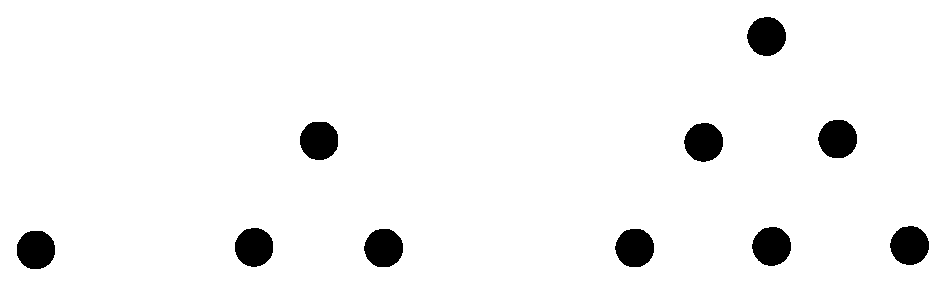
\includegraphics[width=4cm]{figs/pyth-triangles.eps}
  \caption{%
    Talen 1, 3 och 6 representerade med Pythagoreiska trianglar.
  }\label{fig:pyth-triangles}
\end{figure}
\begin{figure}
  \centering
  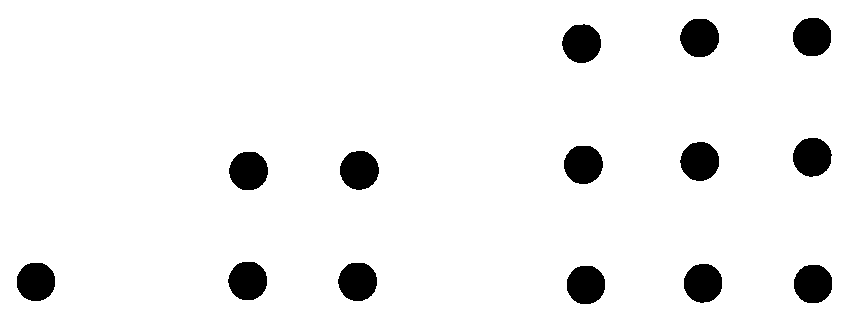
\includegraphics[width=4cm]{figs/pyth-squares.eps}
  \caption{%
    Talen 1, 4 och 9 representerade med Pythagoreiska kvadrater.
  }\label{fig:pyth-squares}
\end{figure}
Tal som kunde representeras som en triangel kallade de följaktligen för 
triangulära tal\index{triangulära tal} och tal som kunde representeras som 
kvadrater kallades för kvadratiska tal\index{kvadratiska tal}.
Ett resultat som fascinerade dem var att varje kvadratiskt tal kunde 
konstrueras genom additionen av två triangulära tal.
Ett annat, det som gavs som \cref{eq:pyth-square} ovan, är hur nästa 
kvadratiska tal återfinns; \( (n+1)^2 \) är det kvadratiska tal som följer 
\(n^2\) och \(2n + 1\) är antalet prickar som måste läggas till längs kanterna.
\begin{exercise}
  Undersök om det finns ett liknande uttryck för triangulära tal.
\end{exercise}
\begin{exercise}
  För vilka triangulära tal gäller att om två triangulära tal adderas är 
  resultatet ett kvadratiskt?
\end{exercise}

Fermats och Eulers resultat som omnämndes redan i \cref{Introduktion} är ett 
mycket intressant talteoretiskt resultat.
Det är fortfarande historiskt, dock modernt i jämförelse med ovan nämnda 
resultat.
Vi kommer att behandla Fermats och Eulers satser senare i detta kapitel.

Ytterligare ett resultat, ett olöst sådant, är Goldbachs förmodan.
Denna förmodan uttalades av Chrisitan Goldbach (1690--1794)~\cite{goldbach} och 
säger att varje naturligt tal kan skrivas som en summa av primtal.
Begreppet primtal är centralt för talteorin och vi kommer strax att återkomma 
till dessa.


%%%%%%%%%%%%%%%%%%%%%%%%%%%%%%%%%%%%%%%%%%%%
% DELBARTHET
%%%%%%%%%%%%%%%%%%%%%%%%%%%%%%%%%%%%%%%%%%%%
\section{Delbarhet}
Ett av de centrala begreppen inom talteorin är delbarheten hos de hela 
talen.
Vi inleder avsnittet med att definiera vad vi menar med detta.
\begin{definition}[Delbarhet]\index{delbarhet}\index{delare}\index{äkta delare}
  Vi säger att ett tal \(a\in\Z\) delar ett tal \(b\in\Z\) om det finns ett tal 
  \(q\in\Z\) sådant att \(b = qa\).
  Vi skriver då \(a\mid b\), vilket utläses som \emph{\(a\) delar \(b\)}.
  På motsvarande sätt har vi \(a\nmid b\) för \emph{\(a\) delar inte \(b\)}.
  Om dessutom \(a\neq b\) sägs \(a\) vara en \emph{äkta delare} till \(b\).
\end{definition}
\begin{example}
  Vi har att \(2\mid 4\) eftersom att \(4 = 2\cdot 2\), två är dessutom en äkta 
  delare.
  Tre är däremot inte en delare till fyra, så \(3\nmid 4\).
  Vi har att \(3\mid 12\) eftersom att \(12 = 3\cdot 2^2\), tre är dessutom en 
  äkta delare till \(12\).
  Vi har har \(12\mid 12\) eftersom att \(12 = 1\cdot 12\), men \(12\) är dock 
  inte en äkta delare till \(12\).
\end{example}
\begin{exercise}\label{xrc:delare}
  Undersök hur olika tal delar varandra och se om ni finner något samband.
\end{exercise}

För att underlätta i kommande bevis ger vi först ett antal fundamentala lemman 
om egenskaperna för delbarhet.
\begin{lemma}\label{lem:divtransitiv}
  Om \(a\mid b\) och \(b\mid c\), då måste även \(a\mid c\).
\end{lemma}
\begin{proof}
  Låt \(b = xa\) och \(c = yb\), då måste \(c = yxa\) och följaktligen måste 
  \(a\mid c\).
\end{proof}
\begin{lemma}\label{lem:divassoc}
  Om \(a\mid b\) och \(a\mid c\), då måste \(a\mid xb + yc\) för alla heltal 
  \(x\) och \(y\).
\end{lemma}
\begin{exercise}
  Bevisa \cref{lem:divassoc}.
\end{exercise}
\begin{lemma}\label{lem:divdistnondiv}
  Om \(a\mid b\) och \(a\nmid c\), då måste \(a\nmid b+c\).
\end{lemma}
\begin{exercise}
  Bevisa \cref{lem:divdistnondiv}, ett förslag är att tillämpa 
  \cref{lem:divassoc}.
\end{exercise}
\begin{exercise}
  Diskutera och förklara varför \(3\mid 6\) men \(3\nmid 5\), \(3\nmid 2\) och 
  \(3\nmid 1\) då \(6 = 5 + 1 = 4 + 2 = 3 + 2 + 1 = 3 + 3\).
\end{exercise}
\begin{lemma}\label{lem:divnoll}
  Om \(ab\neq 0\) och \(a\mid b\) och \(b\mid a\), då måste \(a = b\) eller \(a 
  = -b\).
\end{lemma}
\begin{proof}
  Låt \(a = xb\) och \(b = ya\), då måste \(b = yxb\).
  Eftersom att \(b\neq 0\) måste \(yx = 1\) och således är \(x\) och \(y\) 
  antingen båda \(1\) eller båda \(-1\).
\end{proof}
\begin{lemma}\label{lem:divneg}
  Om \(a\mid b\), då måste \(-a\mid b\), \(-a\mid -b\) och \(a\mid -b\).
\end{lemma}
\begin{exercise}
  Bevisa \cref{lem:divneg}.
\end{exercise}
\begin{exercise}
  Diskutera innebörden av de olika lemmorna.
\end{exercise}

När vi nu är bekanta med begreppet delare ska vi introducera 
divisionsalgoritmen.
Denna ger oss ett verktyg för att dela heltal med varandra och är faktiskt den 
första typen av division som introduceras i svensk skola, den introduceras 
redan i årskurs 1--3 i grundskolan.

\begin{theorem}[Divisionsalgoritmen]\label{thm:divisionsalgoritmen}\index{divisionsalgoritmen}
  Låt \(b\) vara ett positivt heltal.
  För varje heltal \(a\) finns unika heltal \(q\) och \(r\) sådana att \[a = qb 
  + r,\] där \(0\leq r < b\).
\end{theorem}

Innan vi bevisar att algoritmen är korrekt är det lämpligt att vi bevisar ett 
antal lemman.

\begin{lemma}\label{lem:DisjunktaIntervallAvZ}
  Låt \( i_x = \{y\in\Z \colon xb\leq y < (x + 1)b\} \) beteckna ett intervall 
  för varje \(x\in\Z\).
  Då är \(i_x\) och \(i_{x'}\) disjunkta, det vill säga \(i_x\cap \i_{x'} = 
    \emptyset\).
  Deras union \(\cup_{x\in \Z} i_x = \Z\) utgör hela \(\Z\).
\end{lemma}
\begin{exercise}
  Bevisa ovanstående lemma.
  Arbeta med de två delarna var för sig: bevisa att intervallerna är disjunkta 
  och bevisa att unionen utgör hela \(\Z\).
\end{exercise}

\begin{proof}[Bevis för divisionsalgoritmen]
  Eftersom att intervallerna \[
    i_x = \{y\in\Z \colon xb\leq y < (x + 1)b\}
  \] för alla \(x\in\Z\) är disjunkta och deras union \(\cup_{x\in \Z} i_x = 
    \Z\) utgör hela \(\Z\) (\cref{lem:DisjunktaIntervallAvZ}) måste det finnas 
  ett heltal \(q\) sådant att \(qb\leq a < (q+1)b\).
  Låt \(r = a - qb\), då får vi från \(qb\leq a < (q + 1)b\) att \[ r = a - qb 
  < (q + 1)b - qb = b.\]

  För att visa att \(q\) och \(r\) är unika antar vi att det existerar något 
  \(q^\prime\neq q\) och något \(r^\prime\neq r\) sådana att \(a = q^\prime 
  b + r^\prime\).
  Då måste \[0 = (qb + r) - (q^\prime b + r^\prime) = (q - q^\prime)b + (r 
  - r^\prime)\] och således \[ (q - q^\prime)b = -(r - r^\prime) = r^\prime 
  - r.\]
  Följaktligen har vi att \(b\) delar \(r^\prime - r\), men detta är omöjligt 
  då \(0\leq r, r^\prime < b\) ger \(-b < r - r^\prime < b\).
  Vi har då visat att \(r = r^\prime\) och \(q = q^\prime\) och således att 
  \(q\) och \(r\) är unika.
\end{proof}

\begin{definition}
  Vi kallar \(q\) och \(r\) i \cref{thm:divisionsalgoritmen} för
  \emph{heltalskvoten till \(a\) vid division med \(b\)} respektive
  \emph{resten till \(a\) vid division med \(b\)}.
\end{definition}

Notera att enligt våra definitioner stämmer det överens att ett tal \(a\) delar 
ett tal \(b\) då resten är noll.

\begin{exercise}\label{xrc:KvotenMindre}
  Bevisa följande.
  Låt \(a\) och \(b\) vara två heltal.
  Heltalskvoten \(q\) till \(a\) vid division med \(b\) är strikt mindre än 
  \(a\) om \(b\) är strikt större än ett.
\end{exercise}
\begin{exercise}
  Visa att om \(a^2 = 4q + r\) är \(r\) lika med noll eller ett.
\end{exercise}

%%%%%%%%%%%%%%%%%%%%%%%%%%%%%%%%%%%%%%%%%%%%
% PRIMTAL OCH SAMMANSATTA TAL
%%%%%%%%%%%%%%%%%%%%%%%%%%%%%%%%%%%%%%%%%%%%
\subsection{Primtal och sammansatta tal}
Det självklara steget för den nyfikne efter att vi definierat delare är att 
undersöka vilka tal som delar varandra (\cref{xrc:delare}).
Detta har fascinerat matematiker sedan tusentals år tillbaka.
Vi vet redan att både Pythagoréerna och Euklides studerat detta.
Vi ska därför fortsätta genom att definiera ytterligare ett fundamentalt 
begrepp.
\begin{definition}\index{primtal}\index{sammansatt tal}
  Ett tal \(p > 2\) större än två vars enda positiva delare är \(1\) och \(p\) 
  sägs vara ett \emph{primtal}.
  Om \(p\) har fler delare kallas det för ett \emph{sammansatt tal}.
\end{definition}

Följande sats, aritmetikens fundamentalsats, visades i princip av Euklides.
I den sjunde boken av hans \emph{Elementa} finns två satser som tillsammans
kan visa aritmetikens fundamentalsats.
Den visades dock först i sin helhet av Carl Friedrich Gauss (1777--1855) i sin
bok tillika doktorsavhandling \emph{Disquisitiones 
  Arithmeticae}~\cite{Kline1990mtf3}, som är latin för \emph{utforskning av
tal}.
Gauss skrev boken 1798 när han var 20 år gammal och den publicerades 1801.
Den handlar om talteori och sammanfattar tidigare resultat, men introducerar
även nya.
Aritmetikens fundamentalsats var ett av dessa nya resultat.
\begin{theorem}[Aritmetikens 
  fundamentalsats]\label{thm:AritmetikensFundamentalsats}\index{aritmetikens 
    fundamentalsats}
  Ett heltal \(n\in\Z\) kan skrivas som en unik produkt av primtal och \(1\)
  eller \(-1\).
\end{theorem}
%\begin{proof}
%  % XXX Komplettera med bevis för Aritmetikens fundamentalsats
%  \dots
%\end{proof}
\begin{exercise}
  Beviset kan delas upp i två delar.
  Bevisa först att varje tal antingen är ett primtal eller kan skrivas som en 
  produkt av primtal.
  Detta görs enklast med ett induktionsbevis.
  Bevisa därefter att om ett tal kan skrivas som en produkt av primtal, då är 
  den produkten unik sånär som på ordningen av faktorerna\footnote{%
    Det vill säga \(a\cdot b\) och \(b\cdot a\) räknas som samma produkt.
  }.
  Antag att \(p_1p_2\dotsb p_m = q_1q_2\dotsb q_n\), bevisa att \(m = n\) och 
  att varje \(p_i\) motsvarar ett \(q_j\).
\end{exercise}

Följande sats har varit känd under väldigt lång tid, den är idag känd som
Euklides sats.
Eventuellt var satsen känd även tidigare, men den skrevs ned av Euklides i
den nionde boken av \emph{Elementa}.
Euklides \emph{Elementa} bestod av totalt 13 böcker och användes som lärobok
i matematik ända fram till 1900-talet.
\begin{theorem}[Euklides sats]\index{Euklides sats}
  Det finns oändligt många primtal.
\end{theorem}
\begin{proof}
  Vi antar att det finns ändligt många primtal, då kan vi beteckna mängden av 
  alla primtal som \(P = \{p_1, p_2, \dotsc, p_n\}\).
  Vi tittar på ett heltal \(m\).
  Enligt aritmetikens fundamentalsats, 
  \cref{thm:AritmetikensFundamentalsats}, kan vi välja detta \(m\) sådant 
  att \(m = p_1\cdots p_n\) är produkten av alla primtal.
  Vi låter dessutom \(q=m+1\).
  Eftersom att \(q > p_i\) för alla \(i\) kan inte \(q\) vara ett element i
  \(P\), och därför är \(q\) inte ett primtal.
  Då finns det igen enligt aritmetikens fundamentalsats ett primtal \(p\) som 
  delar \(q\).
  Eftersom att \(p\) är ett primtal måste enligt vårt antagande \(p = p_j\) för 
  något \(j\), och alltså måste \(p\) dela \(m\).
  Men om \(p\) delar både \(m\) och \(q = m + 1\), då måste \(p\) även dela
  \(q - m = 1\).
  Då detta är omöjligt får vi en motsägelse och det måste alltså finnas
  oändligt många primtal.
\end{proof}


\section{Fermats och Eulers satser}\label{sec:fermateuler}
% XXX Skriv avsnitt om Fermats och Eulers satser
[Avsnittet är ej ännu färdigskrivet.]

\begin{theorem}[Fermats lilla sats]\index{Fermats lilla sats}
  Låt \(p\) vara ett primtal.
  För alla heltal \(a\) som ej är delbara med \(p\) har vi att resten till 
  \(a^{p-1}\) vid division med \(p\) är \(1\).
\end{theorem}
\begin{proof}
  % XXX Komplettera bevis för Fermats lilla sats
  \dots
\end{proof}

\begin{exercise}
  Låt \(p\) vara ett primtal.
  Visa att för alla \(a < p\) mindre än \(p\) har vi att resten till \(a^p\) 
  vid division med \(p\) är \(a\).
\end{exercise}

\begin{definition}
  % XXX Ange definition för största gemensamma delare
  Största gemensamma delare \dots
\end{definition}
\begin{definition}
  % XXX Ange definition för relationen relativt prima
  Relativt prima \dots
\end{definition}

\begin{theorem}[Eulers sats]\index{Eulers sats}
  Låt \(n\) vara ett positivt heltal.
  För varje tal \(a\) sådant att \(a\) och \(n\) är relativt prima har vi att 
  \[ a^{\phi(n)} \congruent 1 \pmod n. \]
\end{theorem}
\begin{proof}
  % XXX Komplettera bevis för Eulers sats
  \dots
\end{proof}


\section{Stora problem inom talteorin}

Fermats stora sats, eller Fermats förmodan, ställde Fermat upp år 1637.
Han påstod sig ha ett elegant bevis, men att detta inte rymdes i marginalen där 
han skrev kommentaren.
Satsen ges här som sats istället för förmodan då den bevisades 1995 av Andrew 
Wiles (1953--).

\begin{theorem}[Fermats förmodan]\index{Fermats förmodan}\index{Fermats stora 
    sats|see{Fermats förmodan}}
  Det finns inga heltal \(a\), \(b\) och \(c\) sådana att \(a^n + b^n = c^n\) 
  för något heltal \(n\) större än två.
\end{theorem}

Då Wiles bevis är betydligt längre än denna text i sin helhet återges inte 
beviset här.
Dessutom krävs det många års universitetsstudier i matematik för att kunna 
tillgodogöra sig det.

Ett annat stort problem, men som fortfarande saknar bevis, är \emph{Goldbachs 
förmodan}.
Som nämndes i inledningen ställdes denna förmodan upp av Goldbach under 
1700-talet.
\begin{conjecture}[Goldbachs förmodan]\index{Goldbachs förmodan}
  Varje naturligt tal kan skrivas som en summa av primtal.
\end{conjecture}
En enklare version av Goldbachs förmodan bevisades år 2013, det resultatet 
säger att alla udda tal kan skrivas som en summa av primtal.

Nu till några begrepp som vi fått från Fermat och Marin Mersenne (1588--1648).
\begin{definition}
  Ett tal på formen \(F_n = 2^{2^n} + 1\) kallas för ett \emph{Fermattal}.
  Ett tal på formen \(M_p = 2^p - 1\), där \(p\) är ett primtal kallas för ett 
  \emph{Mersennetal}.
  När \(M_p\) i sin tur är ett primtal kallas det för ett 
  \emph{Mersenneprimtal}.
\end{definition}
Fermat hävdade att alla Fermattal är primtal.
Han hade dock inget bevis och det visar sig att det enbart är de fyra första 
som är primtal, det femte visade Euler att det är ett sammansatt tal.
Det är enbart dessa fyra Fermattal som vi känner till som är primtal, det är 
okänt om det finns några fler~\cite{Laksov2005kou}.
\begin{conjecture}
  Det finns oändligt många Fermattal.
\end{conjecture}
Det finns däremot desto fler kända Mersenneprimtal, vi vet dock inte om det 
finns oändligt många.
\begin{conjecture}
  Det finns oändligt många Mersenneprimtal.
\end{conjecture}

Låt oss nu gå vidare till en annan typ av tal som också fascinerat matematiker 
genom tiderna, nämligen perfekta tal.
\begin{definition}
  Ett heltal \(n\) sägs vara ett \emph{perfekt tal}\index{perfekt tal} om \(n\) 
  är summan av alla sina äkta positiva delare.
\end{definition}
\begin{example}
  Talet \(6\) är ett perfekt tal då \(6 = 3\cdot 2\cdot 1 = 3 + 2 + 1\).
\end{example}

Euler bevisade åtminstone ett resultat om perfekta tal, det ges som följande 
sats.
\begin{theorem}
  Alla jämna perfekta tal \(n\) kan skrivas på formen \(p(p + 1)/2\), där \(p\) 
  är ett Mersenneprimtal.
\end{theorem}
Det finns dock mycket som vi inte vet om perfekta tal.
Följande två hypoteser är fortfarande varken bevisade eller motbevisade.
\begin{conjecture}
  Det finns inga udda perfekta tal.
\end{conjecture}
\begin{conjecture}
  Det finns oändligt många perfekta tal.
\end{conjecture}

För vidare fördjupning inom området talteori rekommenderas
Laksovs \citetitle{Laksov2005kou}~\cite{Laksov2005kou} eller
Shoups \citetitle{ShoupNTB}~\cite{ShoupNTB}.
